\documentclass{article}

\usepackage[utf8]{inputenc}
\usepackage{fancybox,fancyhdr}
\usepackage[T1]{fontenc}
\usepackage[left=1cm,right=1cm, top=2cm,bottom=2cm,bindingoffset=0cm]{geometry}
\usepackage{amsmath, nccmath}
\usepackage[normalem]{ulem}
\usepackage[english,russian]{babel}
\usepackage{amssymb,latexsym,amsmath}
\usepackage{setspace}
\usepackage{graphicx}
\usepackage[export]{adjustbox}
\usepackage{wrapfig}
\usepackage{longtable}
\usepackage{caption}
\usepackage{multirow}
\usepackage{textcomp}
\usepackage{tabularx}
\usepackage{tikz}
\usepackage{lastpage}
\usetikzlibrary{fadings}
\usetikzlibrary{calc, angles, positioning, intersections, arrows.meta, patterns}
\usepackage{esvect}
\usepackage[up,bf,raggedright]{titlesec}
\usepackage{float}
\restylefloat{table}
\graphicspath{{noiseimages/}}

\geometry{a4paper}

\date{}
\fancyhead[L]{}
\fancyhead[C]{}

\fancyfoot[L]{Страница \thepage \; из \pageref{LastPage}}
\fancyfoot[C]{}

\begin{document}
\pagestyle{fancy}

%-------------------------------------------------------------------------------------------------------------------------------------------
%-------------------------------------------------------------------1-----------------------------------------------------------------------
%-------------------------------------------------------------------------------------------------------------------------------------------

\section*{Почему орбиты планет замкнуты}

Нахождение орбиты планеты - это задача о движении тела "вокруг" другого, более массивного неподвижного тела, иначе говоря, частицы во внешнем поле, потенциал которой зависит только от расстояния $r$ до определенной неподвижной точки, координаты которой задаются положением массивного тела в простарстве, такое поле называется \textit{центральным}. Сила
\begin{equation}\label{eq1}
\textbf{F} = -\frac{\partial U(r)}{\partial\textbf{r}} = \frac{dU}{dr} \frac{\textbf{r}}{r}
\end{equation}  
Момент ипульса в такой системе сохраняется, т.е. является интегралом движения:
\begin{equation}\label{eq2}
\textbf{M} = [\textbf{rp}]
\end{equation}
Векторы \textbf{M} и \textbf{r} взаимно перпендикулярны, то \textbf{r} всегда лежит в одной и той же плоскости, то есть траектория движения частицы в центральном поле лежит в одной плоскости.
Введя полярные координаты r и $\phi$, запишем функцию Лагранжа:
\begin{equation}\label{eq3}
L = \frac{m}{2}\left(\dot{r}^2 + r^2 \dot{\varphi}^2\right) - U(r)
\end{equation}
Заметим, что $\varphi$ не входит в явном виде в лагранжеву функцию, поэтому такая обобщенная координата является \textit{циклической} и, в силу уравнения Лагранжа:
\begin{equation}\label{eq4}
\frac{d}{dt} \frac{\partial L}{\partial \dot{\varphi}} = \frac{\partial L}{\partial \varphi} = 0
\end{equation} 
 соответсвующий $p_\varphi = \frac{\partial L}{\partial \dot{\varphi}}= mr^2\dot{\varphi}$ является интегралом движения. Опуская дальнейшие преобразования, мы можем получить зависимость $\varphi(\textbf{r})$:
\begin{equation}\label{eq5}
\varphi = \int \frac{(M/r^2)dr}{\sqrt{2m[E-U(r)] - (M^2/r^2)}} + const,
\end{equation}
где $M = mr^2\dot{\varphi}$ - момент импульса, $E = \frac{m\dot{r}^2}{2} + \frac{M^2}{2mr^2} + U(r)$ - энергия системы.
Стоит заметить, что движение ограничено значениями $r$, при которых $\dot{r} = 0$ (переход от уменьшения к увеличению радиус-вектора и наоборот). Если траектория ограничена $r_\text{min} \leq r$, то она \textit{инфинитна}, если же $r_\text{min} \leq r \leq r_\text{max}$ - она \textit{финитна}. Однако, финитность траектории совсем не означает ее замкнутость. За время, пока радиус-вектор изменяется от $r_\text{min}$ к $r_\text{max}$ и наоборот, $\textbf{r}$ повернется на:
\begin{equation}\label{eq6}
\Delta \varphi = 2 \int_{r_{min}}^{r_{max}} \frac{(M/r^2)dr}{\sqrt{2m[E-U(r)] - (M^2/r^2)}}  
\end{equation}


\begin{figure}[H]
        \centering
        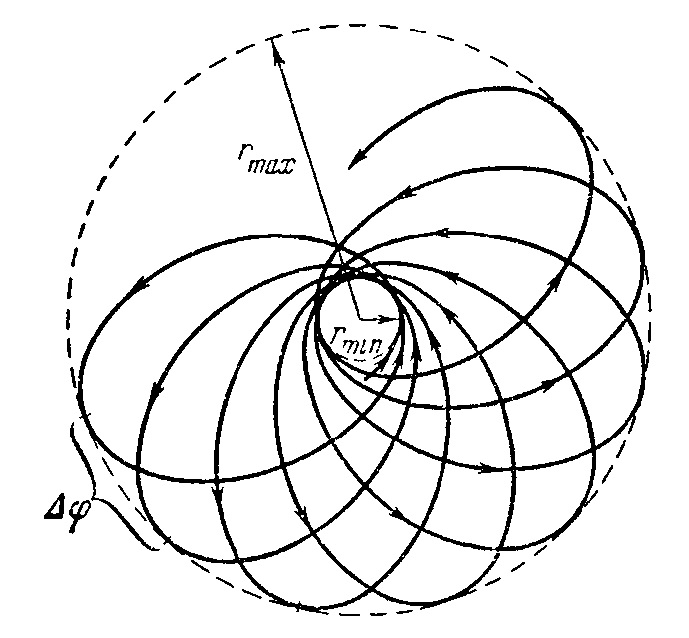
\includegraphics[width=0.5\textwidth]{1.jpg}
\end{figure}
Чтобы орбита замыкалась, $\Delta \varphi = 2\pi \frac{n}{m}$, где $m$ и $n$ - целые числа. В общем виде это не так: при произвольном $U(r)$ $\Delta \varphi$ не обязательно является рациональной частью $\varphi$, но если рассматривать гравитационное поле, интересующее нас в задаче об орбитах планет, то $U(r) \sim \frac{1}{r^2}$ является удовлетворяющим вышеуказанному условию полем. Поэтому орбиты планет замкнуты.

\end{document} 

\begin{wrapfigure}[14]{r}{0.5\linewidth}
        \vspace{-3ex}
        \centering
        \includegraphics[width=\linewidth]{pr4.PNG}
        \label{gal}
\end{wrapfigure}

